\documentclass[12pt]{article}
\usepackage{graphicx} % Required for inserting images
\usepackage{hyperref}
\usepackage[margin=1.27cm]{geometry}
\usepackage{mathptmx, newtxmath}
\usepackage{amsmath}
\usepackage{indentfirst}
\setlength{\parindent}{2em}

\title{Report: MA6217 Problem-Based Assignment 2}
\author{Yang Jiaxin, Matriculation No.: G2605405J}
\date{4/10/2026}

\begin{document}

\maketitle

Check all the codes, Simulink files, images, raw data and report at ntulearn or:

\href{https://github.com/MrOxOrOxen/ntu/tree/ma6217/PBA2}{github.com/MrOxOrOxen/ntu/tree/ma6217/PBA2}.

\section{Task 1}

The objective of the energy-based controller is to drive the pendulum energy $E$ towards a desired energy level $E_d$. The pendulum energy is defined as
$$E = \frac{1}{2}ml^2\dot{\theta}^2 + mgl(cos\theta-1)$$

where the upright stationary configuration corresponds to $E=0$. The proposed Lyapunov function and control law are
$$V = \frac{1}{2}(E-E_d)^2$$
$$\ddot{p}=-k(E-E_d)\dot{\theta}cos\theta$$

Since $V \ge 0$ and $V=0$ means $E=E_d$, $V$ provides a measure of the error between the current energy and the desired energy.

Differentiating $V$ gives
$$\dot{V} = (E-E_d)\dot{E}$$

The derivative of the energy is
$$\dot{E} = ml^2\dot{\theta}\ddot{\theta} - mlgsin\theta\dot{\theta}$$

For $\gamma=0$, the pendulum dynamics are
$$ml^2\ddot{\theta}-mlcos\theta\ddot{p}-mglsin\theta=0$$

Therefore
$$\dot{E} = ml\dot{\theta}cos\theta\ddot{p}$$
$$\dot{V} = ml(E-E_d)\dot{\theta}cos\theta\ddot{p} = -mlk(E-E_d)^2\dot{\theta}^2cos^2\theta \le 0$$

Hence, the Lyapunov function is non-increasing under the proposed controller.

The condition $\dot{V} = 0$ occurs if $E=E_d$ or $\dot{\theta}=0$ or $cos\theta=0$. The latter two cases must be examined separately as required in the assignment.

If $\dot{\theta}=0$, the control law gives $\ddot{p}=0$, and the pendulum dynamics therefore reduce to $\ddot{\theta}=\frac{g}{l}sin\theta$. Unless $sin\theta=0$, the angular acceleration is non-zero. Hence, $\dot{\theta}=0$ is generally only an instantaneous condition and the pendulum immediately starts moving again.

If $\theta = \pm\frac{\pi}{2}$, then $cos\theta=0$, so $\ddot{p}=0$. However, $\ddot{\theta}=\frac{g}{l}sin\theta=\pm\frac{g}{l}\ne0$. Therefore, the pendulum cannot remain at $\theta = \pm \frac{\pi}{2}$, and these positions are not equilibria.

A special invariant case occurs when the pendulum is exactly stationary in the downward configuration:
$$\theta=(2n+1)\pi, \dot{\theta}=0$$

In this case, $\ddot{p}=0$ and $\ddot{\theta}=0$. Therefore, an exactly downward and stationary pendulum remains at this non-target equilibrium. The pure energy controller cannot initiate swing-up from this condition without a perturbation.

If the desired energy is selected as $E_d=0$, then $E=E_d$. At an equilibrium, $\dot{\theta}=0$, so $mgl(1-cos\theta)=0$, which gives $\theta=2n\pi$. Thus, the desired equilibrium for $E_d=0$ is
$$\theta=2n\pi, \dot{\theta}=0$$

or equivalently the upright and stationary pendulum.

By LaSalle's invariance principle, trajectories approach the largest invariant set contained in $\dot{V}=0$. Except for the exactly stationary downward equilibrium discussed above, the closed-loop motion approaches the desired energy level $E=E_d$. For $E_d=0$, the corresponding target equilibrium is the upright configuration.

\section{Task 2}

\subsection{Closed-loop autonomous system}

Let $\omega = \dot{\theta}$. From the pendulum dynamics, we get
$$ml^2\ddot{\theta} = mlcos\theta\ddot{p} + mglsin\theta$$

Substituting
$$\ddot{p} = -k(E-E_d)\dot{\theta}cos\theta$$

gives the closed loop system
\[
\begin{cases}
\dot{\theta} = \omega\\
\dot{\omega} = \frac{g}{l}sin\theta - \frac{k}{l}(E-E_d)\omega cos^2\theta
\end{cases}
\]

where $E = \frac{1}{2}ml^2\omega^2 + mgl(cos\theta-1)$. Since the right-hand side depends only on the states $\theta$ and $\omega$, the closed-loop system is autonomous.

Task 2 does not explicitly specify a value of $E_d$. However, the overall objective of the assignment is pendulum swing-up, and task 1 showed that the upright stationary configuration corresponds to $E_d=0$. Therefore, $E_d=0$ is used for the following phase-plane analysis.

\subsection{Equilibrium points}

At an equilibrium, $\dot{\theta}=0$ and $\dot{\omega}=0$. Since $\dot{\theta}=\omega$, it follows that $\omega_e=0$.

For the second state equation $\dot{\omega}=\frac{g}{l}sin\theta_e$, when $\dot{\omega}=0$, the equation is $sin\theta_e=0$, and hence $(\theta_e, \omega_e) = (n\pi, 0)$.

The equilibria can be divided into two groups $\theta_e = 2n\pi$ and $\theta_e = (2n+1)\pi$, which corresponds to the upright and downward configuration.

\subsection{Phase portrait}

Below is the figure of the phase portrait for $k=0.2$ and $E_d=0$.

\begin{figure}[htbp]
    \centering
    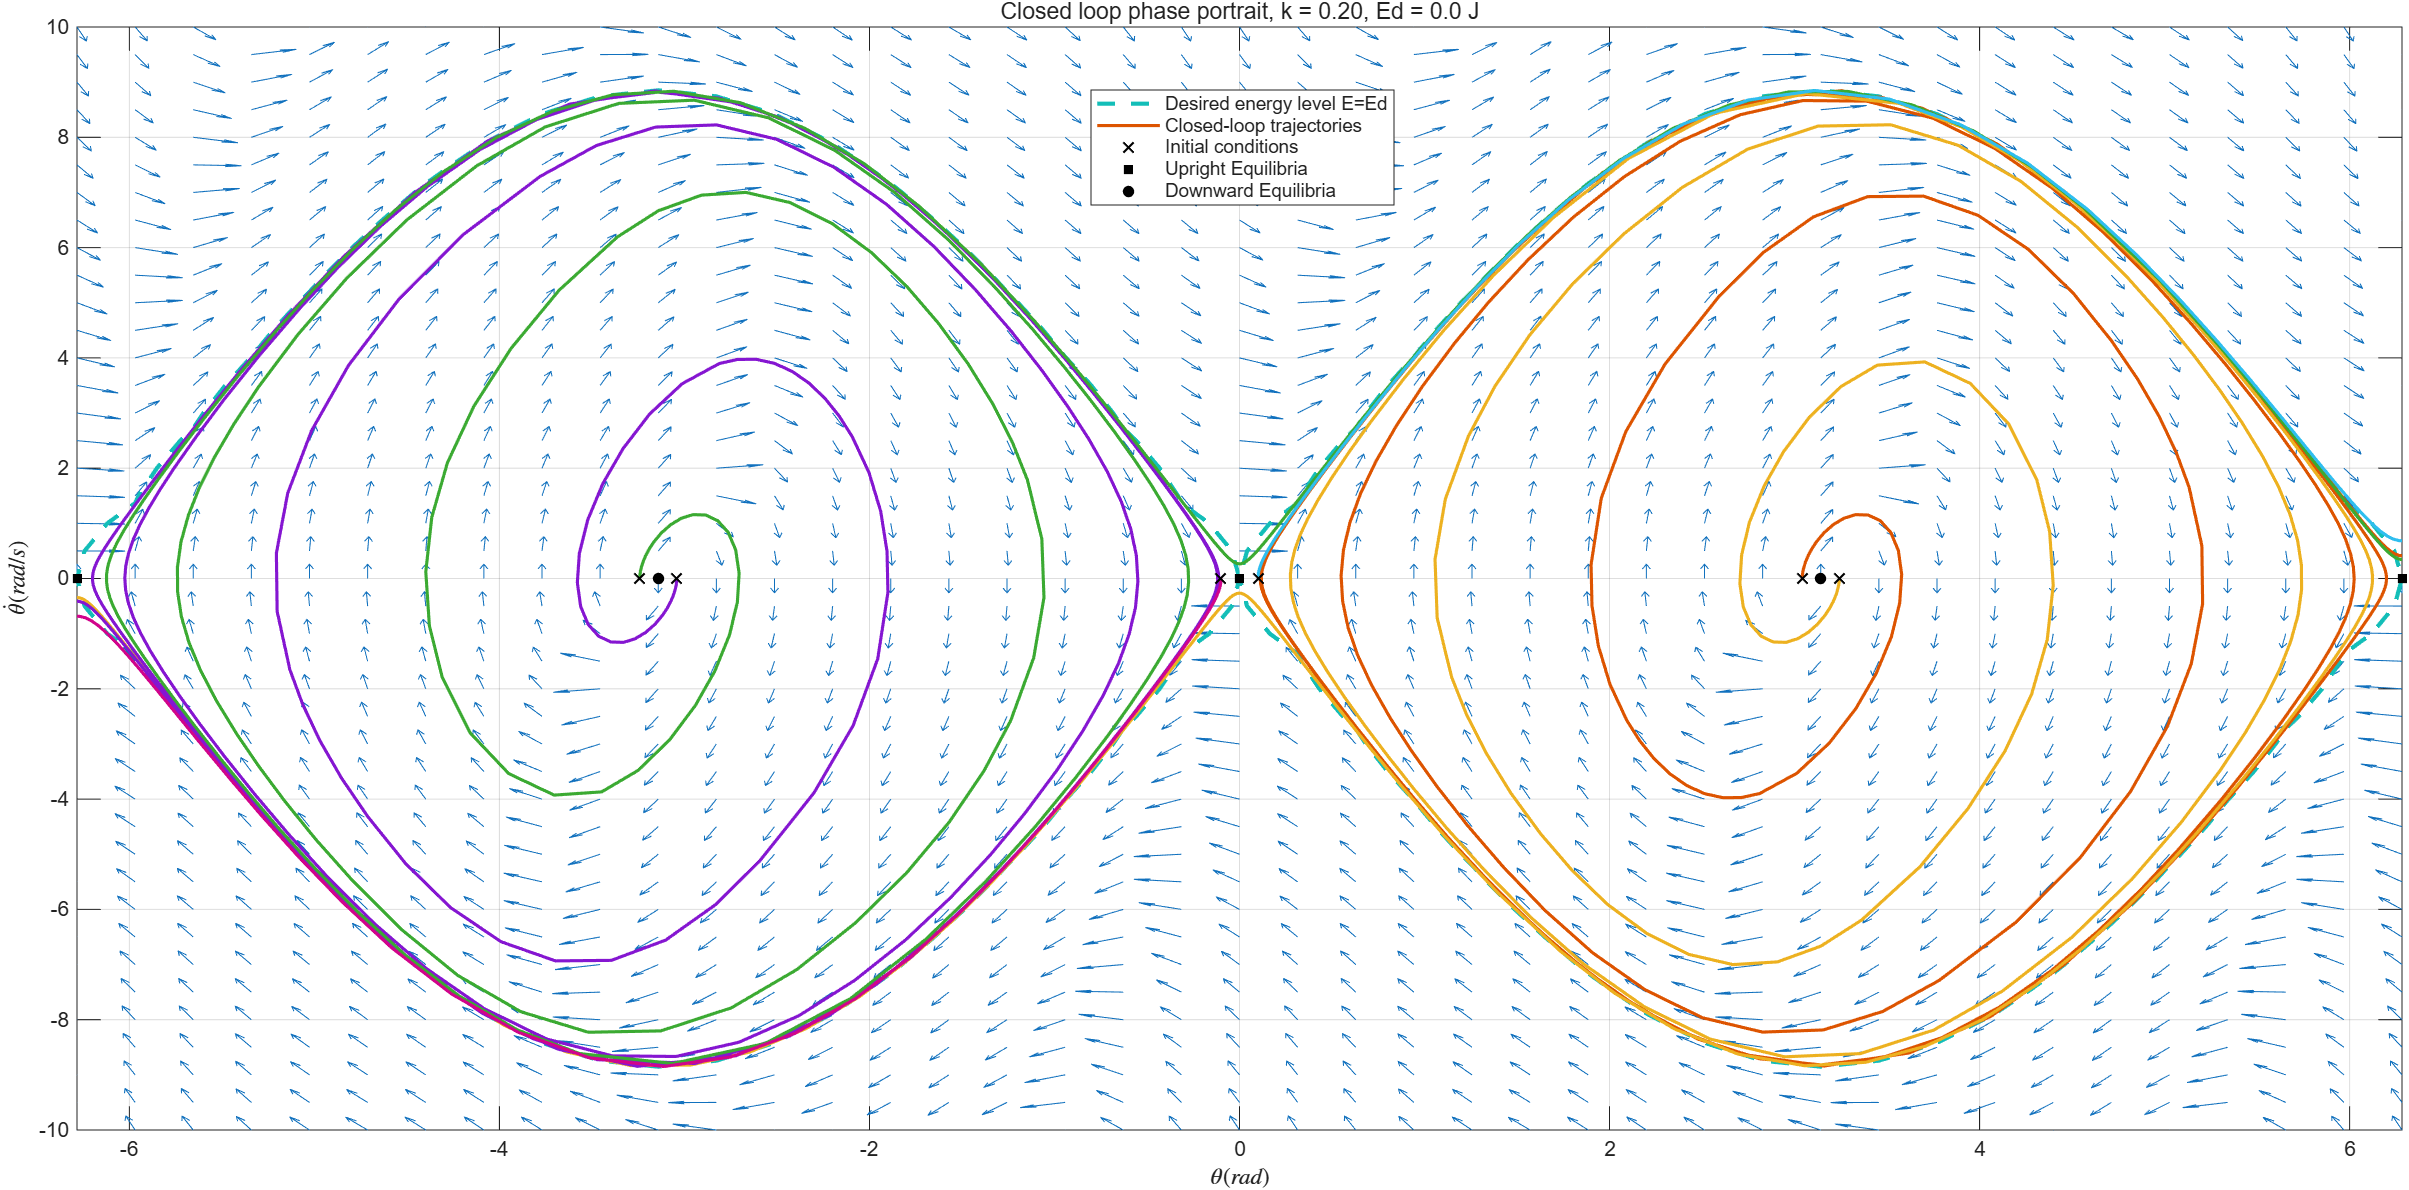
\includegraphics[width=0.9\linewidth]{src/fig1.png}
    \caption{Phase portrait for k=0.2 and Ed=0}
\end{figure}

The phase portrait shows that trajectories starting close to the downward equilibria at $\theta=\pm\pi$ spiral outwards. This indicates that the downward equilibria are unstable. Physically, this corresponds to the energy controller progressively increasing the pendulum oscillation amplitude during swing-up.

As the motion develops, the trajectories approach the desired energy level $E=E_d=0$. The dashed curve in the phase portrait represents all states $(\theta,\dot{\theta})$ that have the desired pendulum energy. The upright equilibria at $\theta=2n\pi,\ \dot{\theta}=0$ lie on this curve.
The phase portrait also shows that the upright equilibria do not attract all nearby trajectories, which is consistent with the linearisation result that they are saddle points and therefore unstable.

\subsection{Linearization of the equilibria}

The nonlinear closed-loop system can be written as $\dot{x}=f(x)$, where $x=\begin{bmatrix}\theta \\ \omega\end{bmatrix}$.

The Jacobian evaluated at an equilibrium $(\theta_e, 0)$ is
$$
A = \begin{bmatrix}
0 & 1 \\
\frac{g}{l}cos\theta_e & -\frac{k}{l}(E_e-E_d)
\end{bmatrix}
$$

where $E_d=0$ and $k=0.2$.

\subsubsection{Upright equilibrium}

For $\theta_e = 2n\pi$, $E_e = E_d = 0$, then $A_{up} = \begin{bmatrix}
    0 & 1 \\ 19.6 & 0
\end{bmatrix}$, and the eigenvalues are $\lambda_1 = 4.4272$ and $\lambda_2 = -4.4272$. Since one eigenvalue is positive and the other is negative, the upright equilibrium is a saddle point and is unstable. This is consistent with the phase portrait, where some trajectories may approach the upright point along a particular direction, while trajectories with a component in the unstable direction move away from it.

\subsubsection{Downward equilibrium}

When $\theta_e = (2n+1)\pi$, the energy is $E_e = -2mgl = -9.8J$, and $A_{down} = \begin{bmatrix}
    0 & 1 \\ -19.6 & 3.92
\end{bmatrix}$. The eigenvalues are $\lambda_{1,2} = 1.96 \pm 3.9697i$, which form a complex-conjugate pair with positive real part. Hence, the downward equilibrium is an unstable focus. This agrees with the outward spiral observed around the downward equilibria in the phase portrait.

\subsection{Selection of k}

To investigate the effect of the controller gain, the value of $k$ is tested among 0.05, 0.1, 0.2, 0.3, 0.4 and 0.5. Since $A_{up}$ and its eigenvalues are independent of $k$ when $E_d=0$, the upright equilibrium remains a saddle point with eigenvalues $\lambda = \pm4.4272$. Therefore, the selection of $k$ mainly affects the transient behavior around the downward equilibrium and the rate of energy regulation.

The eigenvalues of the downward equilibrium were:

\begin{table}[h]
    \centering
    \begin{tabular}{ccc}
         \hline
         $k$ & Eigenvalues & Equilibrium type \\
         \hline
         0.05 & $0.49 \pm 4.4000i$ & unstable focus \\
         0.1 & $0.98 \pm 4.3174i$ & unstable focus \\
         0.2 & $1.96 \pm 3.9697i$ & unstable focus \\
         0.3 & $2.94 \pm 3.3100i$ & unstable focus \\
         0.4 & $3.92 \pm 2.0576i$ & unstable focus \\
         0.5 & $2.80, 7.00$ & unstable node \\
         \hline
    \end{tabular}
    \caption{Eigenvalues of the downward equilibrium}
\end{table}

\begin{figure}
    \centering
    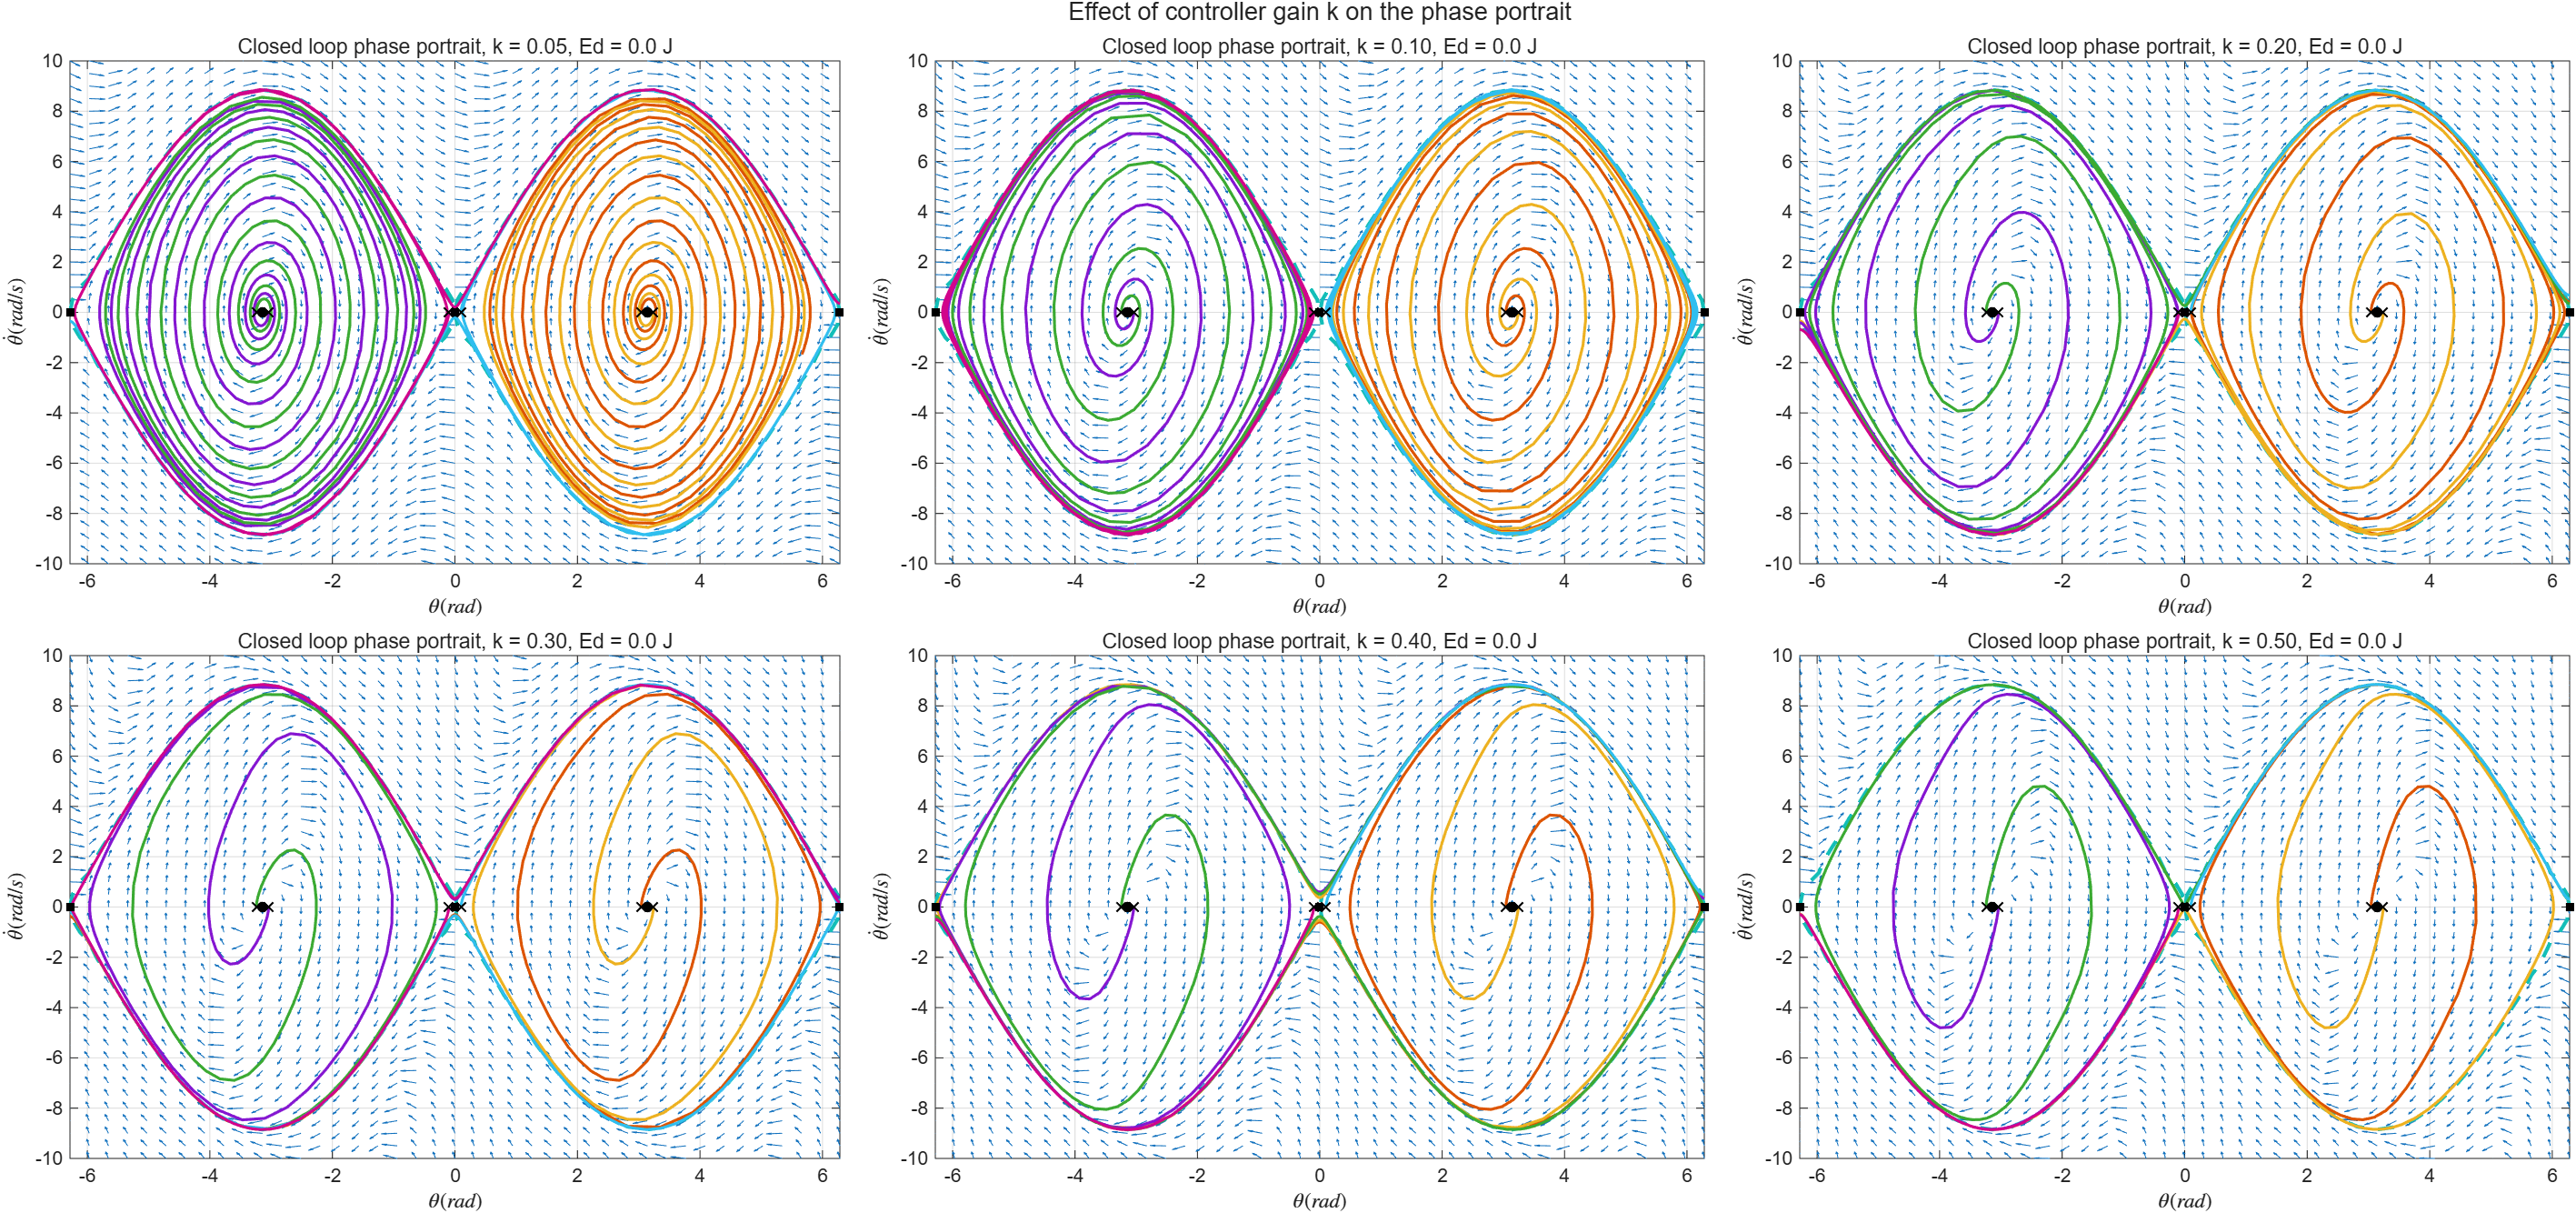
\includegraphics[width=1\linewidth]{src/fig2.png}
    \caption{Phase portrait for different k values (legend in Figure 1)}
\end{figure}

As from Figure 2, for small values of $k$ such as $k=0.05$, trajectories leave the downward equilibrium slowly and undergo many outward oscillations before approaching the desired energy level. Increasing $k$ increases the rate of energy regulation and produces a more aggressive closed-loop response.

The downward equilibrium changes from an unstable focus to an unstable node when the eigenvalues become real. This means for the equation $\lambda^2 - 19.6k\lambda + 19.6=0$, there is $(19.6k)^2 - 4\times19.6 = 0$, which gives approximately $k = 0.452$. It means if $0 < k < 0.452$, $k$ gives an unstable focus, whereas for $k>0.452$, it is an unstable node.

Based on the phase portraits and eigenvalue analysis, $k=0.2$ was selected as a suitable controller gain. It provides a moderate rate of departure from the downward equilibrium while retaining a smooth oscillatory swing-up behaviour. Smaller values result in noticeably slower energy regulation, while larger values produce increasingly aggressive behaviour.

\section{Task 3}

\subsection{Nonlinear cart-pendulum model}

Unlike tasks 1 and 2, where the cart acceleration $\ddot{p}$ was treated as the control input, the input to the plant in task 3 is the applied force $F$. The model was constructed directly from the nonlinear equations of motion given in the assignment.

When $\gamma=0$, the system equations are:
$$(M+m)\ddot{p}-mlcos\theta\ddot{\theta}+mlsin\theta\dot{\theta}^2 = F - c\dot{p}$$
$$ml^2\ddot{\theta} - mlcos\theta\ddot{p} - mglsin\theta = 0$$

And therefore
$$\ddot{\theta} = \frac{cos\theta\ddot{p}+gsin\theta}{l}$$

Substituting this expression into the cart equation gives
$$\ddot{p} = \frac{F - c\dot{p}+mgsin\theta cos\theta - mlsin\theta \dot{\theta}^2}{M+m-mcos^2\theta}$$

\subsection{Simulink implementation}

The nonlinear acceleration equations were implemented using a MATLAB Function block. The block takes $F, \dot{p}, \theta, \dot{\theta}$ as inputs and calculates $\ddot{p}$ and $\ddot{\theta}$. Two cascaded integrators were used for the cart motion, and another two cascaded integrators were used for the pendulum motion. The states $\dot{p}, \theta, \dot{\theta}$ were fed back to the MATLAB Function block to evaluate the nonlinear dynamics continuously during the simulation.

\begin{figure}[htbp]
    \centering
    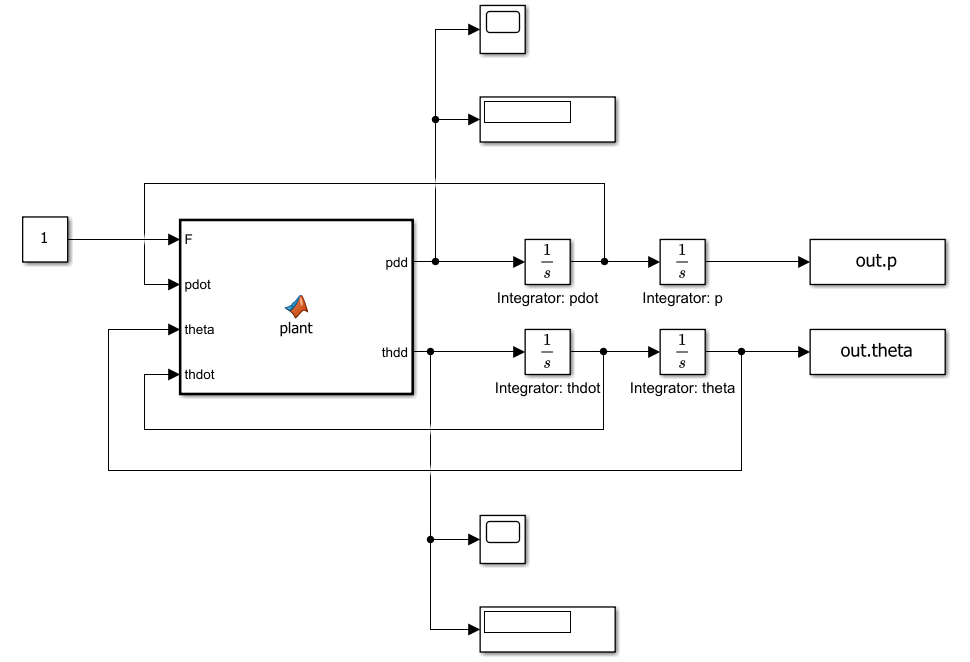
\includegraphics[width=0.7\linewidth]{src/fig3.png}
    \caption{Simulink of task 3}
\end{figure}

\subsection{Model validation}

To verify that the Simulink model reproduces the original equations correctly, a test condition with a known initial configuration and known applied force was used as suggested in the assignment. The initial conditions were $p(0)=0, \dot{p}(0)=0, \theta(0)=0, \dot\theta(0)=0, F=1N$. Through calculation, we get $\ddot{p}(0)=0.2m/s^2$ and $\ddot{\theta}(0)=0.4rad/s^2$. The values obtained directly from the Simulink model were $\ddot{p}(0)=0.2m/s^2$ and $\ddot{\theta}(0)=0.4rad/s^2$, which agree exactly with the analytical calculations.

\subsection{Simulation response}

The model was then simulated for 2 seconds under the same constant force $F=1N$.

\begin{figure}[htbp]
    \centering
    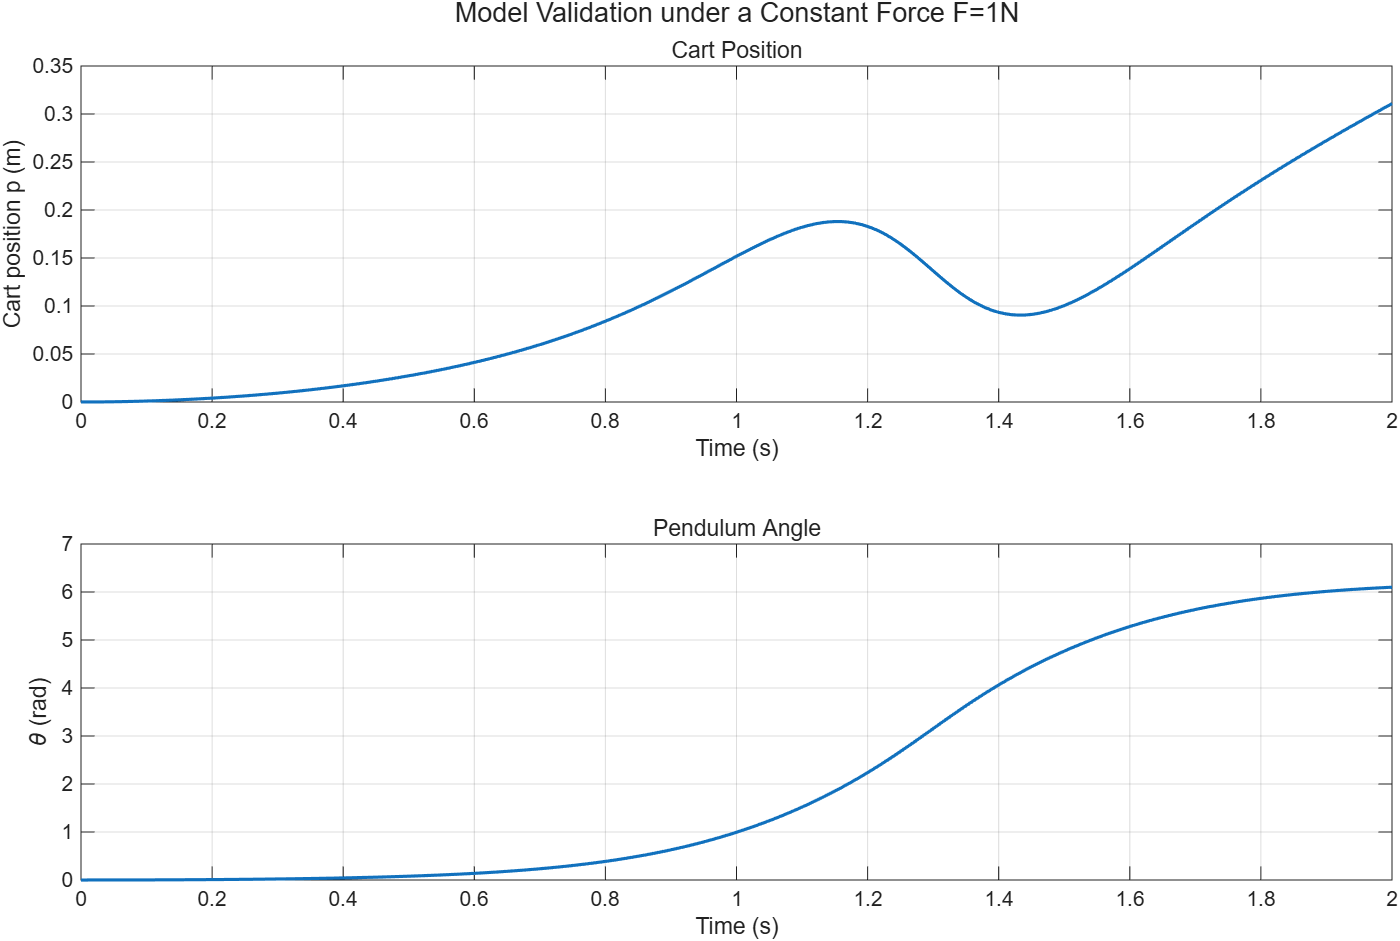
\includegraphics[width=0.9\linewidth]{src/fig4.png}
    \caption{Simulation response of task 3}
\end{figure}

The cart initially moves in the positive direction under the applied force. Because the pendulum and cart are dynamically coupled, the cart motion is influenced by the pendulum motion and is therefore not simply a uniformly accelerating trajectory.

The pendulum angle also increases from its initial upright position. This is expected because the upright equilibrium is unstable, and the horizontal acceleration of the cart produces a non-zero initial angular acceleration. Over the 2-s simulation interval, the pendulum angle increases to approximately one full revolution.

The trajectory is therefore consistent with the nonlinear coupled dynamics of the cart–pendulum system. Together with the exact agreement between the analytical and simulated initial accelerations, the results confirm that the Simulink model has been implemented correctly.

\section{Task 4}

\subsection{Swing-up controller design}

The objective of task 4 is to apply the Lyapunov energy-based controller developed in task 1 to the complete nonlinear cart-pendulum model developed in task 3. In contrast to tasks 1 and 2, where the cart acceleration $\ddot{p}$ was treated as the control input, the actual input to the Simulink plant must be the applied force $F$. The effect of changing the controller gain $k$ must also be investigated.

From task 1, the desired cart acceleration is $\ddot{p_d} = -k(E-E_d)\dot{\theta}cos\theta$, where $E = \frac{1}{2}ml^2\dot{\theta}^2+mgl(cos\theta-1)$. For swing-up to the upright configuration, $E_d=0$.

From task 3:
$$\ddot{p} = \frac{F-c\dot{p}+mgsin\theta cos\theta - mlsin\theta \dot{\theta}^2}{M+m-mcos^2\theta}$$

To make the actual cart acceleration follow the acceleration required by the Lyapunov controller, the condition $\ddot{p} = \ddot{p_d}$ is imposed. So we get
$$F = -(M+m-mcos^2\theta)k(E-E_d)\dot{\theta}cos\theta+c\dot{p}-mgsin\theta cos\theta+mlsin\theta\dot{\theta}^2$$

This force command allows the Lyapunov acceleration-based controller derived in task 1 to be applied to the force-input nonlinear plant developed in task 3.

\subsection{Simulink implementation}

A separate MATLAB Function block was used to implement the swing-up controller. The controller takes $\dot{p}, \theta, \dot{\theta}, k$ as inputs and calculates the pendulum energy $E$, the desired cart acceleration $\ddot{p_d}$ and the corresponding applied force $F$.

The calculated force $F$ is then directly applied to the input of the nonlinear plant developed in task 3. The resulting states are fed back to both the plant and the swing-up controller, forming the closed-loop system.

\begin{figure}[htbp]
    \centering
    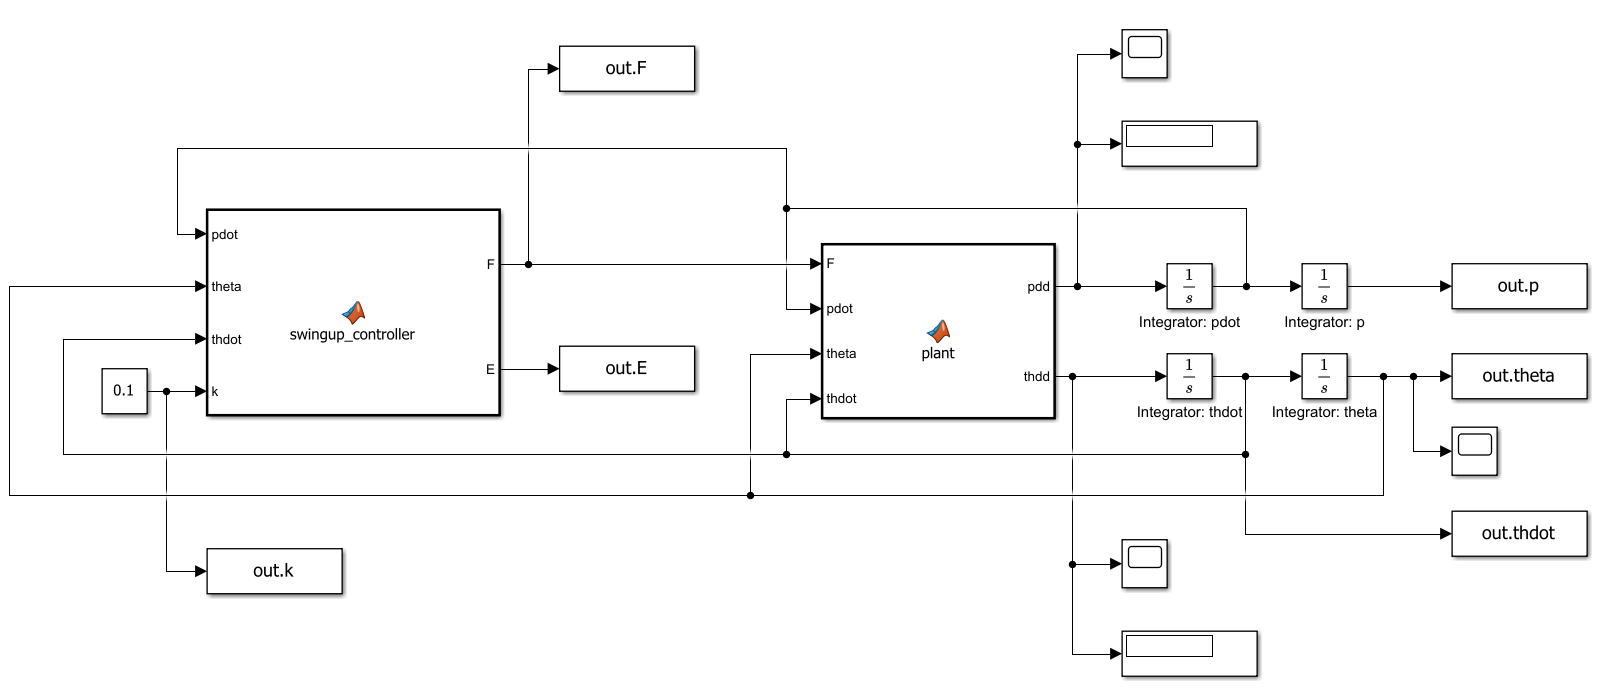
\includegraphics[width=1\linewidth]{src/fig5.png}
    \caption{Simulink of task 4}
\end{figure}

\subsection{Initial condition for swing-up}

An exactly stationary downward pendulum corresponds to $\theta(0)=\pi$ and $\dot{\theta}(0)=0$. We have calculated in task 1 that at this condition, $\ddot{p_d}=0$, so the system remains exactly at the downward equilibrium. Therefore, the pure energy controller cannot initiate swing-up from the exactly stationary downward configuration without a perturbation.

To avoid this invariant equilibrium while still representing a pendulum initially very close to the downward configuration, the simulation was initialized with $\theta(0) = \pi - 0.01 rad$ and $p(0)=0, \dot{p}(0)=0, \dot{\theta}(0)=0$.

\subsection{Swing-up response for k = 0.2}

The controller was first tested using $k=0.2$ which had previously been selected as a suitable moderate gain in task 2.

\begin{figure}[htbp]
    \centering
    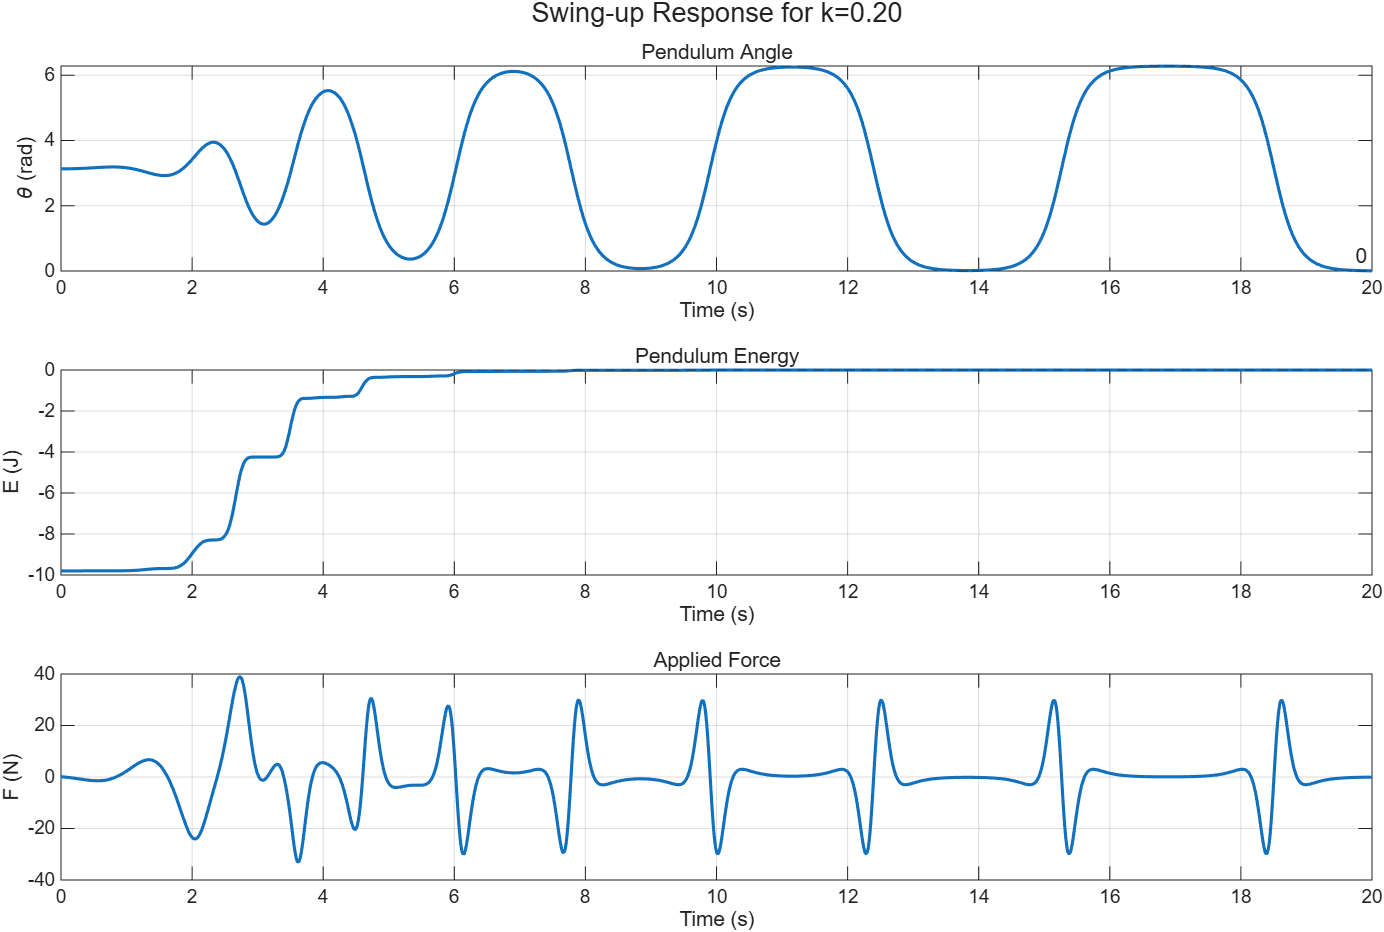
\includegraphics[width=0.9\linewidth]{src/fig6.png}
    \caption{Simulation result of k=0.2 in task 4}
\end{figure}

The pendulum initially starts close to the downward configuration $\theta \approx \pi$, and the controller progressively increases the pendulum energy, causing the oscillation amplitude to grow. The pendulum therefore swings increasingly close to the upright configurations $\theta=2n\pi$.

The energy initially has approximately the downward-equilibrium value $E(0) \approx -9.8 J$. During the swing-up process, the controller raises the energy towards the desired value $E_d=0$. For $k=0.2$, the energy first satisfies $|E| < 0.05J$ at $t=7.70s$. The final simulated energy after 20 s was $E(20) = -1.8 \times 10^{-5} J$, which is very close to the desired energy. The corresponding peak control force was $max|F| = 38.92N$ and the maximum absolute cart displacement was $max|p| = 0.546m$.

The pendulum repeatedly approaches the upright configurations as the energy approaches zero. However, the energy controller alone does not asymptotically stabilize the upright equilibrium. This is consistent with the result from task 2, where the upright equilibrium was shown to be a saddle point. Therefore, the controller performs the swing-up function, while a separate balancing controller would be required if permanent stabilization at the upright position were desired.

\subsection{Effect of changing k}

To investigate the effect of the controller gain $k$, simulations were performed for $k=0.1,0.2,0.4$ using the same initial conditions and simulation duration. We considered three quantitative measurements: the first time for which $|E|<0.05J$, the maximum absolute applied force $max|F|$, and the maximum absolute cart displacement over the 20-s simulation $max|p|$. The simulation results are summarized below.

\begin{figure}
    \centering
    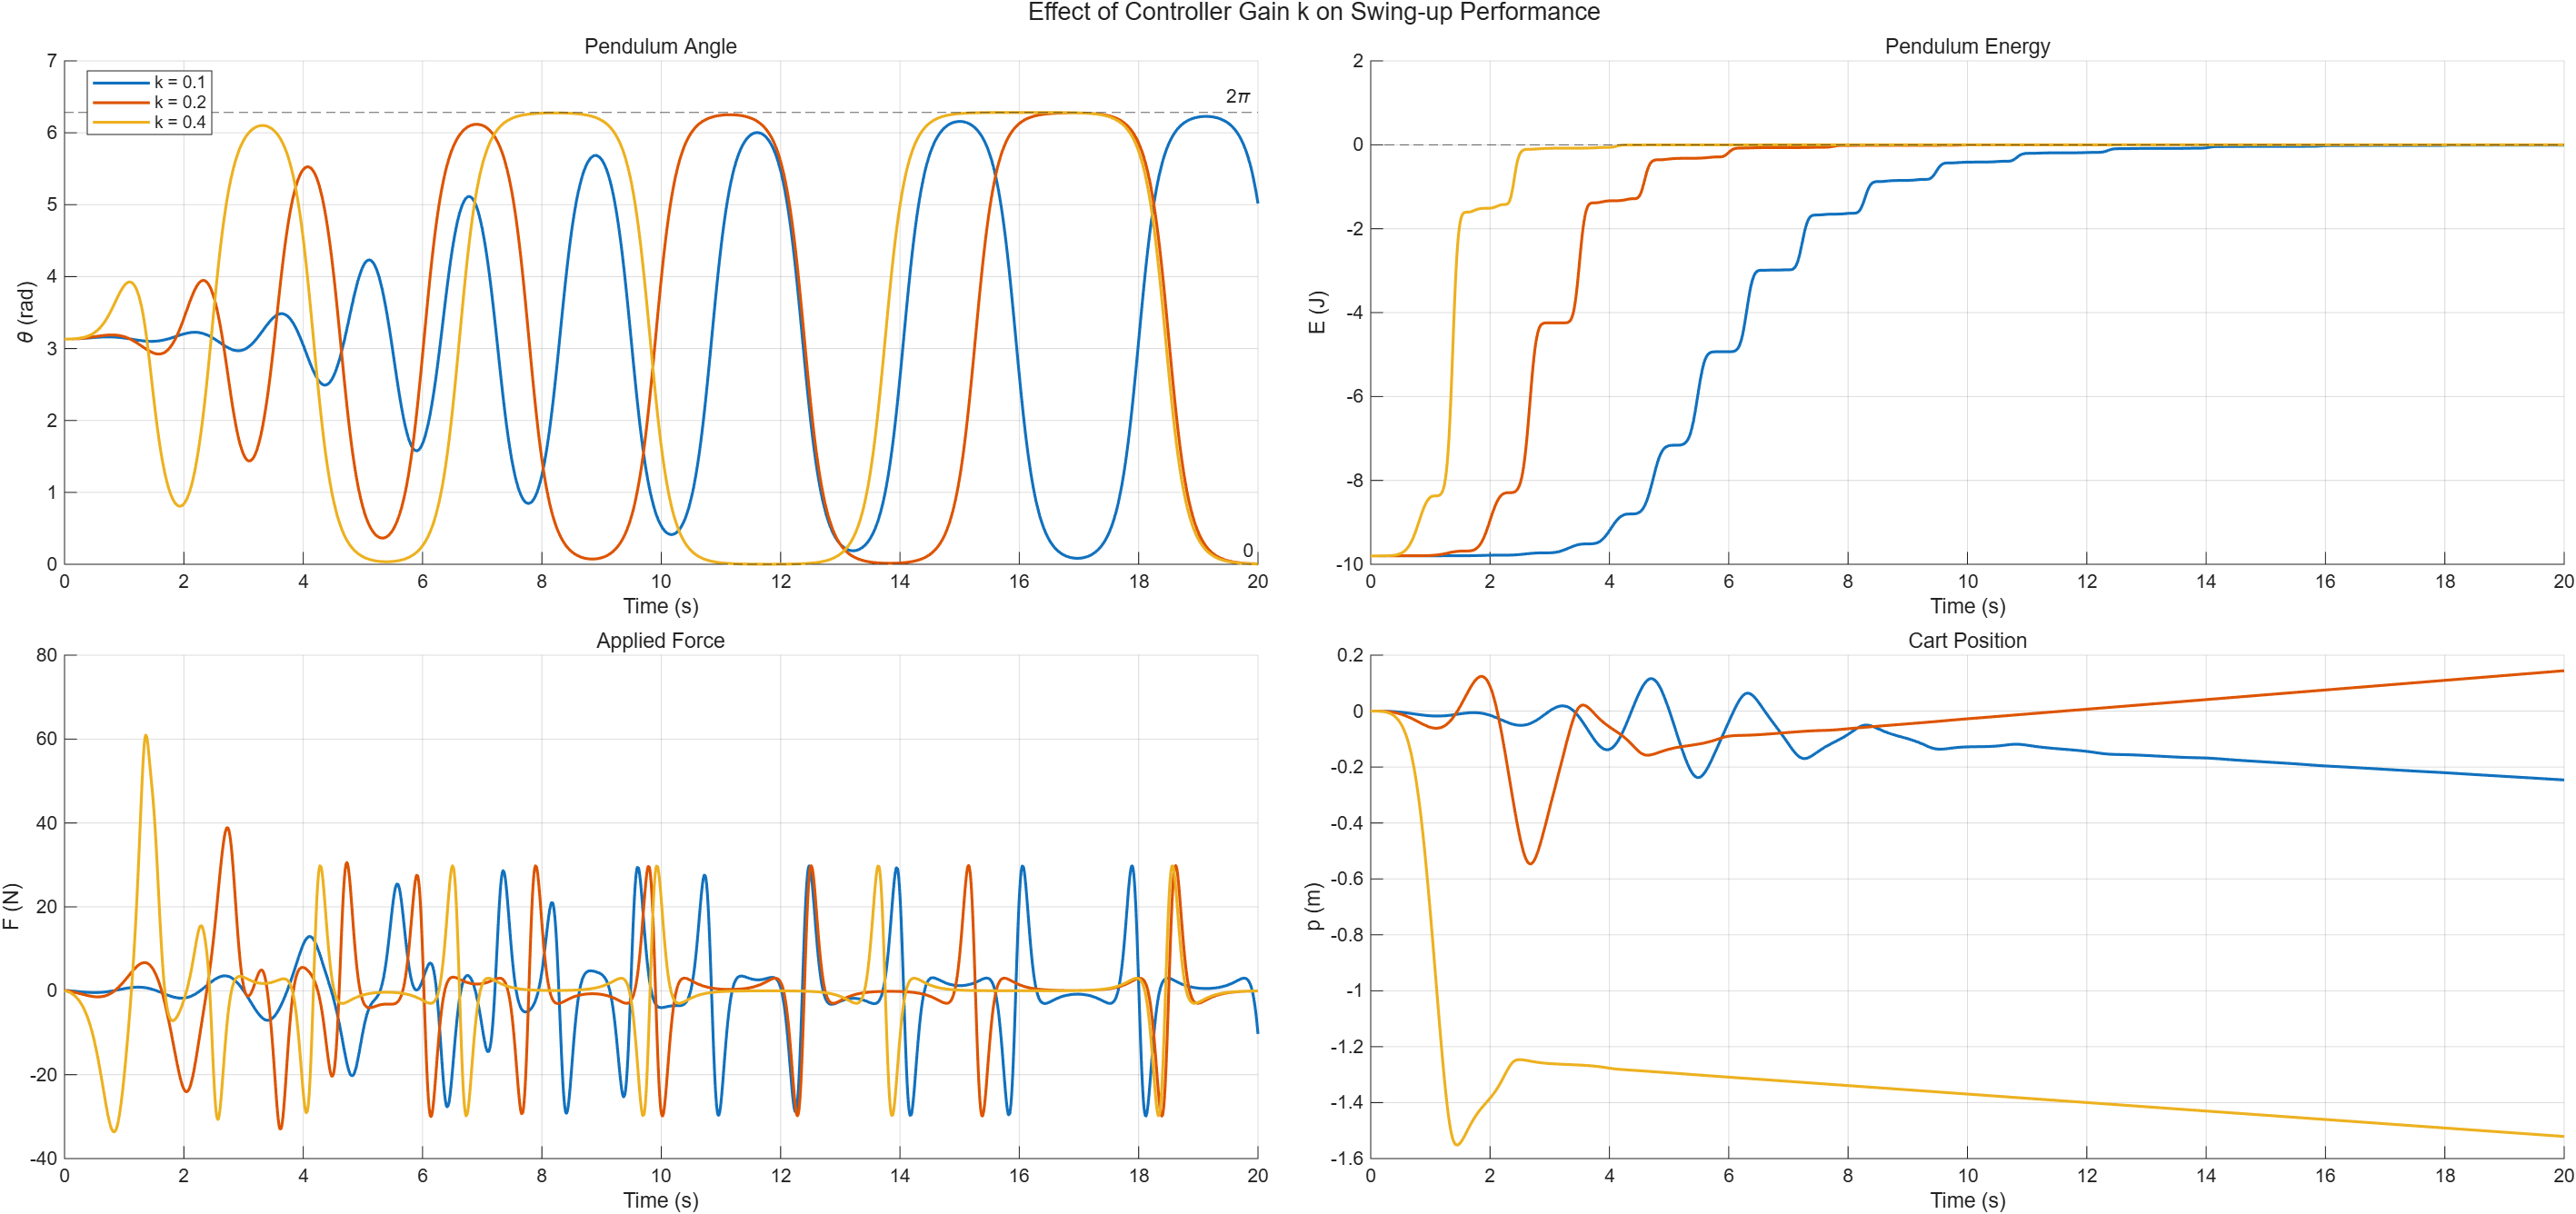
\includegraphics[width=0.9\linewidth]{src/fig7.png}
    \caption{Simulation results for different k values}
\end{figure}

\begin{table}[h]
    \centering
    \begin{tabular}{ccccc}
         \hline
         $k$ & First time $|E|<0.05J$ (s) & $max|F|$ (N) & $max|p|$ (m) & Final $E$ (J) \\
         \hline
         0.1 & 14.11 & 29.87 & 0.246 & -0.00693 \\
         0.2 & 7.70 & 38.92 & 0.546 & -0.000018 \\
         0.4 & 4.08 & 60.99 & 1.552 & $\approx$ 0 \\
         \hline
    \end{tabular}
    \caption{Simulation results for different k values}
\end{table}

For $k=0.1$, the energy rises relatively slowly towards the desired level. The first time for which $|E|<0.05J$ is 14.11 s. However, this case requires the lowest peak force 29.87 N and the smallest cart displacement 0.246 m. Thus, the response is relatively slow but mild.

For $k=0.4$, the target energy region is reached much more rapidly, after only 4.08 s. However, the faster energy regulation requires a substantially larger peak force 60.99 N, and the maximum cart displacement increases to 1.552 m. The response is therefore significantly more aggressive.

The intermediate value $k=0.2$ provides a compromise between these two cases, and therefore was selected as an appropriate controller gain. It provides reasonably fast energy regulation without requiring the substantially larger force and cart excursion associated with the higher gain.

\end{document}
